\documentclass[10pt,a4paper]{article}
\usepackage[a4paper, top=2.0cm, bottom=2.2cm, left=2.2cm, right=2.2cm, headsep=0.6cm]{geometry}
\usepackage{fontspec}
\setmainfont{texgyretermes}[Extension=.otf, UprightFont=*-regular, BoldFont=*-bold, ItalicFont=*-italic, BoldItalicFont=*-bolditalic]
\setsansfont{texgyreheros}[Extension=.otf, UprightFont=*-regular, BoldFont=*-bold, ItalicFont=*-italic, BoldItalicFont=*-bolditalic]
\usepackage{babel}
\babelprovide[import, main]{polish}
\usepackage{microtype}
\usepackage{array, booktabs, longtable, tabularx}
\usepackage[table]{xcolor}
\usepackage{graphicx}
\usepackage{enumitem}
\usepackage{parskip}
\usepackage{fancyhdr}
\usepackage{titlesec}
\usepackage[hidelinks]{hyperref}
\emergencystretch=3em
\setlist{itemsep=2pt, topsep=3pt, leftmargin=1.4em}
\definecolor{L1}{HTML}{2A78D6}\definecolor{L2}{HTML}{EB6834}\definecolor{L3}{HTML}{1BAF7A}
\definecolor{L4}{HTML}{EDA100}\definecolor{L7}{HTML}{E87BA4}\definecolor{muted}{HTML}{767A84}
\definecolor{bad}{HTML}{C23030}\definecolor{good}{HTML}{0A8A0A}
\newcommand{\linedot}[1]{\textcolor{#1}{\rule[0.1ex]{0.9ex}{0.9ex}}\,}
\newcommand{\mut}[1]{\textcolor{muted}{#1}}
\titleformat{\section}{\sffamily\large\bfseries}{\thesection.}{0.5em}{}
\titleformat{\subsection}{\sffamily\normalsize\bfseries}{\thesubsection.}{0.5em}{}
\titlespacing*{\section}{0pt}{1.2em}{0.4em}
\titlespacing*{\subsection}{0pt}{0.9em}{0.3em}
\setlength{\LTpre}{4pt}\setlength{\LTpost}{4pt}
\pagestyle{fancy}\fancyhf{}
\renewcommand{\headrulewidth}{0.3pt}
\fancyhead[L]{\sffamily\footnotesize Załącznik nr 2 do wniosku z dnia \makebox[2.4cm]{\dotfill} 2026 r.}
\fancyhead[R]{\sffamily\footnotesize Przesiadki Iława Główna}
\fancyfoot[C]{\sffamily\footnotesize \thepage}
\begin{document}
{\sffamily\footnotesize\bfseries\MakeUppercase{Załącznik nr 2 · analiza rozkładów}}\par\smallskip
{\sffamily\LARGE\bfseries Przesiadki Iława Główna}\par\medskip
{\large Czy autobusy ZKM odjeżdżają spod dworca akurat wtedy, gdy przyjeżdżają pociągi?}\par\medskip
{\small\mut{Dworzec Iława Główna: 106 pociągów w dzień roboczy. Przystanek Dworcowa: linie ZKM 1, 2, 3, 4, 7, 106 odjazdów w dzień roboczy. Stan na 29.09.2026.}}\par\bigskip
\section*{Odpowiedź}
Teza się nie potwierdza dla całej sieci. W dzień roboczy autobus odjeżdża w chwili przyjazdu pociągu przy \textbf{50\,\%} pociągów. Rozkład losowy daje \textbf{47\,\%} (90\,\% wyników losowych: 40\,\%--56\,\%). Wrażenie „uciekającego autobusu” jest prawdziwe, ale wynika z liczby kursów i skupień pociągów, a nie z ułożenia rozkładu. Rozkłady nie są jednak ze sobą skoordynowane: dobrych przesiadek jest tyle samo, ile przy losowym rozkładzie. Wyjątkiem jest \textbf{linia 1} w dni robocze, gdzie takich sytuacji jest więcej niż losowo (22\,\% wobec 16\,\%). Chodzi o kilka wieczornych odjazdów, po których następny kurs jest za 50--100 min. Sobota: wynik jest blisko górnej granicy losowości (35\,\% wobec 27\,\%), ale kursów jest mało i test nie daje pewności.

{\small
\begin{center}\begin{tabular}{@{}p{9.2cm} r p{4.2cm}@{}}\toprule
Wskaźnik & Wartość & Dla porównania \\ \midrule
Pociągi, którym autobus „ucieka” (dzień roboczy) & 50\,\% & losowo 47\,\%; 86 przyjazdów \\
To samo dla linii 1 (dzień roboczy) & 22\,\% & losowo 16\,\% \\
Mediana opóźnienia pociągów PKP Intercity w Iławie & 3 min & POLREGIO: 0 min \\
Ciasne przesiadki z IC na daną linię (czekanie do 14 min), które się udają & 61\,\% & POLREGIO: 93\,\% \\
\bottomrule\end{tabular}\end{center}}
\section{Test tezy: rozkład rzeczywisty na tle losowego}
Dla każdego pociągu sprawdzono, czy autobus odjeżdża w chwili, gdy podróżni jeszcze idą z peronu na przystanek: od 2 min przed przyjazdem do 4 min po przyjeździe. Ten sam wskaźnik policzono 3000 razy dla rozkładu, w którym każdą linię przesunięto o losowy czas od $-30$ do $+30$ min. Szary pas to zakres 90\,\% wyników losowych, pionowa kreska to średnia losowa. Znacznik poza pasem oznacza wynik lepszy (zielony, trójkąt w stronę lepszego wyniku) albo gorszy (czerwony) niż losowo.

\par\medskip\noindent\begin{minipage}{\textwidth}\centering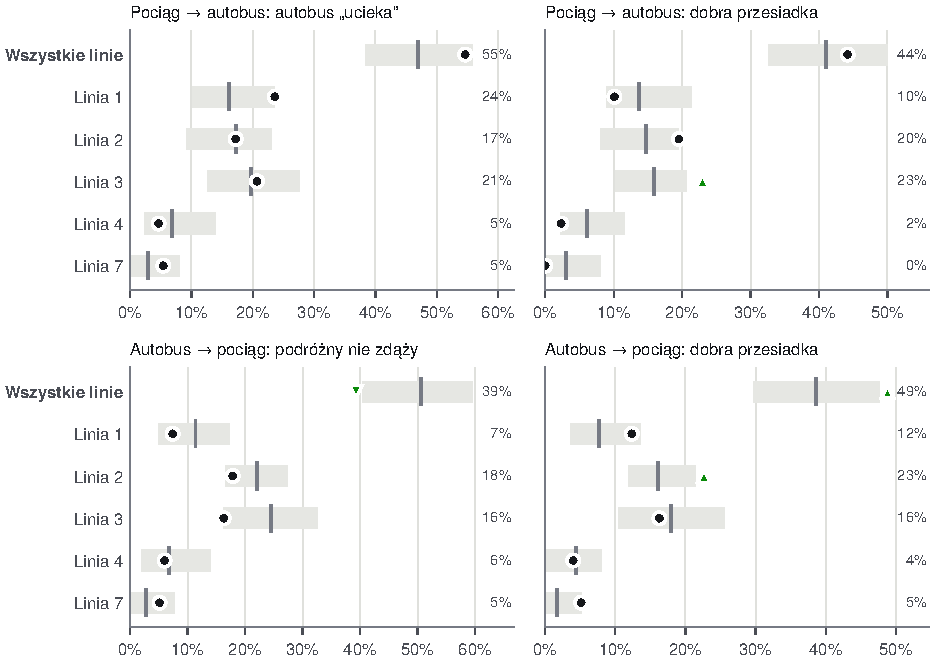
\includegraphics[width=\textwidth]{fig/przesiadki-test.pdf}\par\smallskip
{\small\mut{Rys. 1. Dzień roboczy 30.09.2026. Test obejmuje pociągi w godzinach kursowania danej linii.}}\end{minipage}\par\medskip
Wszystkie linie razem, każdy typ dnia (w nawiasie średnia losowa):
{\small
\begin{center}\begin{tabular}{@{}l r r r r@{}}\toprule
Typ dnia & Pociąg → autobus: ucieka & dobra & Autobus → pociąg: nie zdąży & dobra \\ \midrule
Dzień roboczy & 50\,\% \mut{(47\,\%)} & 67\,\% \mut{(67\,\%)} & 42\,\% \mut{(50\,\%)} & 65\,\% \mut{(64\,\%)} \\
Sobota & 35\,\% \mut{(27\,\%)} & 46\,\% \mut{(41\,\%)} & 25\,\% \mut{(29\,\%)} & 42\,\% \mut{(39\,\%)} \\
Niedziela i święta & 20\,\% \mut{(20\,\%)} & 32\,\% \mut{(30\,\%)} & 14\,\% \mut{(19\,\%)} & 28\,\% \mut{(25\,\%)} \\
\bottomrule\end{tabular}\end{center}}
\section{Kiedy odjeżdża autobus względem przyjazdu pociągu}
Każda para „pociąg -- autobus” w odstępie od $-20$ do $+30$ min, w przedziałach 2-minutowych. Gdyby autobusy uciekały pociągom, słupki w czerwonym polu byłyby wyraźnie wyższe od linii poziomu losowego. Gdyby rozkłady były skoordynowane, wyższe byłyby słupki w zielonym polu.
\par\medskip\noindent\begin{minipage}{\textwidth}\centering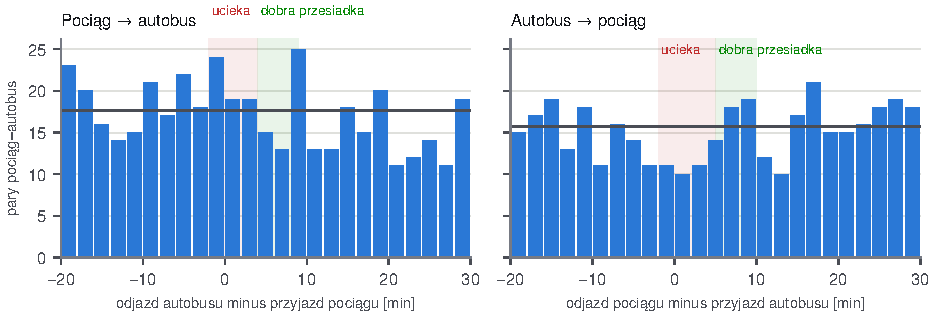
\includegraphics[width=\textwidth]{fig/przesiadki-odstepy.pdf}\par\smallskip
{\small\mut{Rys. 2. Dzień roboczy. Pozioma linia: poziom losowy.}}\end{minipage}\par\medskip
\section{Jeden dzień: przyjazdy pociągów i odjazdy autobusów}
Pionowe kreski to przyjazdy pociągów (długie: IC, EIP, EIC, TLK; krótkie: POLREGIO). Kropki to odjazdy autobusów spod dworca. Czerwona linia łączy pociąg z autobusem, który odjeżdża, zanim podróżni dojdą na przystanek.
\par\medskip\noindent\begin{minipage}{\textwidth}\centering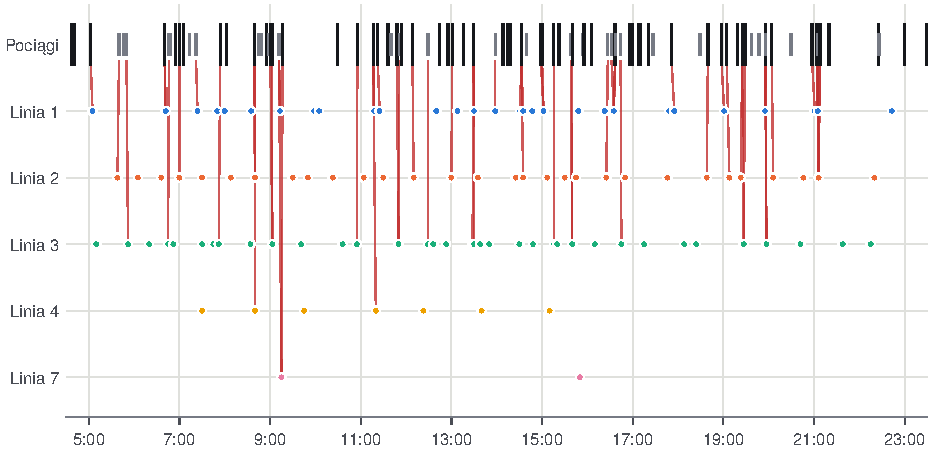
\includegraphics[width=\textwidth]{fig/przesiadki-dzien.pdf}\par\smallskip
{\small\mut{Rys. 3. Dzień roboczy 30.09.2026.}}\end{minipage}\par\medskip
\section{Odjazdy, które „uciekają” pociągom}
Kursy, które odjeżdżają w chwili przyjazdu co najmniej jednego pociągu, a następny kurs tej samej linii jest dopiero po 30 min lub później.
{\footnotesize
\begin{longtable}{@{}l l l p{5.6cm} l r@{}}\toprule
Dzień & Odjazd & Linia & Pociągi w tej chwili & Następny & Czekanie \\ \midrule\endhead
\bottomrule\endfoot
dzień roboczy & 06:42 & \linedot{L1}1 $\to$ Długa & 06:39 IC 5708; 06:44 R 90101 & 07:24 & 42 min \\
dzień roboczy & 06:52 & \linedot{L3}3 $\to$ Nowa Wieś & 06:50 R 90623; 06:52 EIP 5300 & 07:30 & 38 min \\
dzień roboczy & 07:00 & \linedot{L2}2 $\to$ Iława ul. Lipowy Dwór (ogrody) & 06:59 TLK 35171; 06:59 TLK 53104 & 07:30 & 30 min \\
dzień roboczy & 08:40 & \linedot{L2}2 $\to$ Iława ul. Lipowy Dwór (ogrody) & 08:39 IC 1618 & 09:30 & 50 min \\
dzień roboczy & 08:40 & \linedot{L4}4 $\to$ Piaskowa & 08:39 IC 1618 & 09:45 & 65 min \\
dzień roboczy & 09:03 & \linedot{L3}3 $\to$ Nowa Wieś & 09:02 EIP 1503 & 09:41 & 38 min \\
dzień roboczy & 09:13 & \linedot{L1}1 $\to$ Piaskowa & 09:10 R 90730 & 09:58 & 45 min \\
dzień roboczy & 09:15 & \linedot{L7}7 $\to$ Nowa Wieś (pętla, przejazd przez Dworcową) & 09:16 IC 7503 & 15:50 & 395 min \\
dzień roboczy & 10:55 & \linedot{L3}3 $\to$ Nowa Wieś & 10:52 EIP 5402; 10:55 IC 1513 & 11:50 & 55 min \\
dzień roboczy & 11:20 & \linedot{L4}4 $\to$ Piaskowa & 11:16 IC 6115 & 12:23 & 63 min \\
dzień roboczy & 11:50 & \linedot{L3}3 $\to$ Nowa Wieś & 11:48 R 90654 & 12:29 & 39 min \\
dzień roboczy & 12:53 & \linedot{L3}3 $\to$ Nowa Wieś & 12:52 EIP 5352 & 13:28 & 35 min \\
dzień roboczy & 13:00 & \linedot{L2}2 $\to$ Iława ul. Lipowy Dwór (ogrody) & 12:58 IC 1815; 12:58 IC 5114 & 13:35 & 35 min \\
dzień roboczy & 13:58 & \linedot{L1}1 $\to$ Piaskowa & 13:59 R 90200 & 14:31 & 33 min \\
dzień roboczy & 14:35 & \linedot{L2}2 $\to$ Iława ul. Lipowy Dwór (ogrody) & 14:33 IC 5714 & 15:07 & 32 min \\
dzień roboczy & 15:02 & \linedot{L1}1 $\to$ Długa & 15:02 EIP 3553 & 15:48 & 46 min \\
dzień roboczy & 15:40 & \linedot{L3}3 $\to$ Nowa Wieś & 15:38 R 90244 & 16:10 & 30 min \\
dzień roboczy & 16:35 & \linedot{L1}1 $\to$ Długa & 16:34 R 90625; 16:35 IC 1614 & 17:48 & 73 min \\
dzień roboczy & 16:45 & \linedot{L3}3 $\to$ Nowa Wieś & 16:45 R 90656 & 17:15 & 30 min \\
dzień roboczy & 17:55 & \linedot{L1}1 $\to$ Długa & 17:52 EIP 5406 & 19:01 & 66 min \\
dzień roboczy & 18:38 & \linedot{L2}2 $\to$ Iława ul. Lipowy Dwór (ogrody) & 18:39 IC 5702 & 19:08 & 30 min \\
dzień roboczy & 19:01 & \linedot{L1}1 $\to$ Piaskowa & 18:57 IC 1517; 19:01 IC 5110; 19:02 EIP 4503 & 19:55 & 54 min \\
dzień roboczy & 19:55 & \linedot{L1}1 $\to$ Długa & 19:52 EIP 5102 & 21:01 & 66 min \\
dzień roboczy & 20:06 & \linedot{L2}2 $\to$ Iława ul. Lipowy Dwór (ogrody) & 20:04 IC 5320 & 20:46 & 40 min \\
dzień roboczy & 21:05 & \linedot{L1}1 $\to$ Długa & 21:02 EIP 3503; 21:03 R 90113; 21:06 TLK 53170 & 22:43 & 98 min \\
dzień roboczy & 21:06 & \linedot{L2}2 $\to$ Iława ul. Lipowy Dwór (ogrody) & 21:02 EIP 3503; 21:03 R 90113; 21:06 TLK 53170 & 22:20 & 74 min \\
sobota & 05:42 & \linedot{L2}2 $\to$ Iława ul. Lipowy Dwór (ogrody) & 05:40 R 90621; 05:44 R 90205 & 06:15 & 33 min \\
sobota & 06:50 & \linedot{L1}1 $\to$ Długa & 06:50 R 90623 & 07:58 & 68 min \\
sobota & 07:54 & \linedot{L3}3 $\to$ Nowa Wieś & 07:55 IC 1521 & 08:26 & 32 min \\
sobota & 09:00 & \linedot{L3}3 $\to$ Nowa Wieś & 08:57 IC 1857; 08:58 IC 5116 & 09:45 & 45 min \\
sobota & 10:30 & \linedot{L1}1 $\to$ Piaskowa & 10:29 IC 5710 & 11:38 & 68 min \\
sobota & 11:10 & \linedot{L2}2 $\to$ Iława ul. Lipowy Dwór (ogrody) & 11:12 TLK 8328 & 12:01 & 51 min \\
sobota & 11:52 & \linedot{L3}3 $\to$ Nowa Wieś & 11:52 EIP 5302 & 12:35 & 43 min \\
sobota & 12:01 & \linedot{L2}2 $\to$ Iława ul. Lipowy Dwór (ogrody) & 12:02 EIP 3509 & 13:01 & 60 min \\
sobota & 13:01 & \linedot{L2}2 $\to$ Iława ul. Lipowy Dwór (ogrody) & 12:58 IC 1815; 12:58 IC 5114; 13:02 EIP 4507 & 14:11 & 70 min \\
sobota & 13:20 & \linedot{L1}1 $\to$ Długa & 13:16 IC 7515 & 14:53 & 93 min \\
sobota & 14:05 & \linedot{L3}3 $\to$ Nowa Wieś & 14:02 EIP 3507 & 14:35 & 30 min \\
sobota & 14:35 & \linedot{L3}3 $\to$ Nowa Wieś & 14:33 IC 5714 & 15:33 & 58 min \\
sobota & 15:00 & \linedot{L1}1 $\to$ Długa & 14:57 IC 1515; 14:58 IC 8114 & 16:28 & 88 min \\
sobota & 16:37 & \linedot{L2}2 $\to$ Iława ul. Lipowy Dwór (ogrody) & 16:34 R 90625; 16:35 IC 1614; 16:38 R 90225 & 18:10 & 93 min \\
sobota & 17:21 & \linedot{L3}3 $\to$ Nowa Wieś & 17:21 IC 7511 & 19:15 & 114 min \\
sobota & 19:15 & \linedot{L3}3 $\to$ Nowa Wieś & 19:16 IC 6119 & 21:06 & 111 min \\
sobota & 21:06 & \linedot{L3}3 $\to$ Nowa Wieś & 21:02 EIP 3503; 21:03 R 90113; 21:06 TLK 53170 & brak & -- \\
niedziela & 07:58 & \linedot{L3}3 $\to$ Nowa Wieś & 07:55 IC 1521 & 09:16 & 78 min \\
niedziela & 09:00 & \linedot{L2}2 $\to$ Iława ul. Lipowy Dwór (ogrody) & 08:57 IC 1553; 08:58 IC 5116 & 10:51 & 111 min \\
niedziela & 09:16 & \linedot{L3}3 $\to$ Nowa Wieś & 09:16 IC 7503 & 10:00 & 44 min \\
niedziela & 10:51 & \linedot{L2}2 $\to$ Iława ul. Lipowy Dwór (ogrody) & 10:52 EIP 5402 & 12:52 & 121 min \\
niedziela & 10:58 & \linedot{L1}1 $\to$ Długa & 10:55 IC 1513 & 12:13 & 75 min \\
niedziela & 11:46 & \linedot{L3}3 $\to$ Nowa Wieś & 11:48 R 90654 & 12:20 & 34 min \\
niedziela & 12:52 & \linedot{L2}2 $\to$ Iława ul. Lipowy Dwór (ogrody) & 12:52 EIP 5352 & 14:38 & 106 min \\
niedziela & 14:38 & \linedot{L2}2 $\to$ Iława ul. Lipowy Dwór (ogrody) & 14:38 R 55205 & 16:32 & 114 min \\
niedziela & 15:40 & \linedot{L1}1 $\to$ Długa & 15:38 R 90244 & 16:58 & 78 min \\
niedziela & 16:32 & \linedot{L2}2 $\to$ Iława ul. Lipowy Dwór (ogrody) & 16:34 R 90625 & 18:10 & 98 min \\
niedziela & 16:58 & \linedot{L1}1 $\to$ Piaskowa & 16:57 TLK 3829; 16:58 IC 5112 & brak & -- \\
niedziela & 17:21 & \linedot{L3}3 $\to$ Nowa Wieś & 17:21 IC 7511 & 19:15 & 114 min \\
niedziela & 19:15 & \linedot{L3}3 $\to$ Nowa Wieś & 19:16 IC 6119 & 21:08 & 113 min \\
niedziela & 21:08 & \linedot{L3}3 $\to$ Nowa Wieś & 21:06 TLK 53170 & brak & -- \\
\end{longtable}}
\section{Czas oczekiwania na konkretną linię}
Podróżny potrzebuje konkretnej linii, a nie dowolnego autobusu. Mediana czasu od przyjazdu pociągu do odjazdu danej linii oraz od przyjazdu autobusu do odjazdu pociągu, średnio z 4 tygodni rozkładu (30.09.2026--27.10.2026).
{\footnotesize
\begin{longtable}{@{}l l r r r r r@{}}\toprule
Dzień & Linia & Kursy/dzień & Pociąg → linia: mediana & „Ucieka” & Dobra & Linia → pociąg: mediana \\ \midrule\endhead
\bottomrule\endfoot
dzień roboczy & \linedot{L1}1 & 31 & 28 min & 23\,\% & 25\,\% & 34 min \\
dzień roboczy & \linedot{L2}2 & 30 & 22 min & 16\,\% & 31\,\% & 21 min \\
dzień roboczy & \linedot{L3}3 & 36 & 24 min & 15\,\% & 32\,\% & 22 min \\
dzień roboczy & \linedot{L4}4 & 7 & 39 min & 4\,\% & 13\,\% & 35 min \\
dzień roboczy & \linedot{L7}7 & 2 & 34 min & 3\,\% & 8\,\% & 54 min \\
sobota & \linedot{L1}1 & 14 & 28 min & 16\,\% & 20\,\% & 48 min \\
sobota & \linedot{L2}2 & 16 & 32 min & 13\,\% & 17\,\% & 26 min \\
sobota & \linedot{L3}3 & 21 & 32 min & 13\,\% & 24\,\% & 28 min \\
niedziela & \linedot{L1}1 & 12 & 32 min & 8\,\% & 16\,\% & 48 min \\
niedziela & \linedot{L2}2 & 8 & 68 min & 8\,\% & 13\,\% & 73 min \\
niedziela & \linedot{L3}3 & 13 & 38 min & 7\,\% & 13\,\% & 40 min \\
\end{longtable}}
\section{Co robią opóźnienia pociągów}
Rozkład ZKM porównano z faktycznymi czasami pociągów. Dla PKP Intercity są dane z 18 dni (11.09.2026--28.09.2026, źródło: spoznienia.me). Dla wszystkich przewoźników, także POLREGIO, są dane z 4 dni (26.09.2026--29.09.2026, API PKP PLK). Dla autobusów nie ma publicznych danych o faktycznych odjazdach. Przyjęto odchylenie w granicach tolerancji ZKM: od 1 min przed czasem do 3 min po czasie. „Ciasna” przesiadka to taka, w której według rozkładu podróżny czeka na swoją linię najwyżej 14 min.

\subsection*{Opóźnienie przyjazdu do Iławy Głównej}
{\small
\begin{center}\begin{tabular}{@{}l r r r r@{}}\toprule
Kategoria & n & Mediana & 90. percentyl & Ponad 5 min \\ \midrule
EIP \mut{spoznienia.me} & 390 & 3 min & 18 min & 31\,\% \\
EIC \mut{spoznienia.me} & 48 & 6 min & 30 min & 50\,\% \\
IC \mut{spoznienia.me} & 483 & 1 min & 15 min & 22\,\% \\
TLK \mut{spoznienia.me} & 108 & 6 min & 35 min & 54\,\% \\
EIP \mut{API PLK} & 68 & 3 min & 20 min & 25\,\% \\
EIC \mut{API PLK} & 10 & 7 min & 18 min & 60\,\% \\
IC \mut{API PLK} & 88 & 1 min & 16 min & 24\,\% \\
TLK \mut{API PLK} & 19 & 6 min & 28 min & 58\,\% \\
R \mut{API PLK} & 88 & 0 min & 3 min & 3\,\% \\
\bottomrule\end{tabular}\end{center}}
\subsection*{Ciasne przesiadki pociąg → linia, które dochodzą do skutku}
{\small
\begin{center}\begin{tabular}{@{}l r r r@{}}\toprule
Linia & IC (spoznienia.me) & Wszystkie (API PLK) & POLREGIO \\ \midrule
\linedot{L1}1 & 56\,\% \mut{n=249} & 64\,\% \mut{n=44} & 84\,\% \mut{n=11} \\
\linedot{L2}2 & 64\,\% \mut{n=309} & 74\,\% \mut{n=56} & 99\,\% \mut{n=14} \\
\linedot{L3}3 & 67\,\% \mut{n=255} & 77\,\% \mut{n=69} & 93\,\% \mut{n=31} \\
\linedot{L4}4 & 44\,\% \mut{n=60} & 50\,\% \mut{n=8} & -- \\
\linedot{L7}7 & 85\,\% \mut{n=12} & 70\,\% \mut{n=5} & -- \\
\bottomrule\end{tabular}\end{center}}
W przesiadce autobus → pociąg opóźnienie pociągu nie zrywa połączenia, tylko wydłuża czekanie na peronie: średnio z 17,4 do 23,7 min (IC). Połączenie zrywa się tylko wtedy, gdy autobus przyjeżdża z opóźnieniem, a zapas jest mały: w modelu tolerancji ZKM dotyczy to 6\,\% ciasnych przesiadek.
\section{Według jakiego klucza ułożono rozkład?}
ZKM nie publikuje zasad, według których układa rozkład. Dane wykluczają cztery odpowiedzi i wskazują dwa tropy.
\begin{itemize}
\item \textbf{Nie pociągi.} Dopasowanie całej sieci do rozkładu kolejowego jest na poziomie losowym (punkt 1).
\item \textbf{Nie stały takt.} Linie 2 i 3 odjeżdżają średnio co 30--32 min, ale o 18--24 różnych minutach godziny. Odstępy między kursami wynoszą od 2 do 74 min.
\item \textbf{Nie obiegi „na styk”.} Od przyjazdu autobusu na Dworcową do najbliższego odjazdu tej samej linii mija zwykle 21 min (linia 2), 19 min (linia 3) i 12 min (linia 4).
\item \textbf{Nie szkoły.} Rozkład nazywa się szkolnym, ale tylko 4 kursy są oznaczone jako kursujące wyłącznie w dni nauki.
\end{itemize}
\textbf{Trop pierwszy:} obecny rozkład ZKM lepiej pasuje do pociągów IC sprzed korekty rozkładu PKP z 30 sierpnia (druga tabela). \textbf{Trop drugi:} niektóre kierunki są obsłużone lepiej niż losowo, a pociągi z Olsztyna wyraźnie gorzej (pierwsza tabela).

\subsection*{Dopasowanie do grup pociągów w dzień roboczy}
{\footnotesize
\begin{center}\begin{tabular}{@{}p{3.6cm} r l l l l@{}}\toprule
Grupa pociągów & Przyj./odj. & P→A: ucieka & P→A: dobra & A→P: nie zdąży & A→P: dobra \\ \midrule
Działdowo / Warszawa \mut{kierunek} & 26/26 & 50\,\% \mut{(49\,\%)} & 73\,\% \mut{(67\,\%)} & 42\,\% \mut{(49\,\%)} & 73\,\% \mut{(64\,\%)} \\
Jabłonowo / Toruń \mut{kierunek} & 14/14 & 29\,\% \mut{(47\,\%)} & 86\,\% \mut{(68\,\%)} \textcolor{good}{lepiej} & 64\,\% \mut{(51\,\%)} & 57\,\% \mut{(67\,\%)} \\
Malbork / Gdańsk \mut{kierunek} & 28/27 & 46\,\% \mut{(48\,\%)} & 61\,\% \mut{(67\,\%)} & 26\,\% \mut{(51\,\%)} \textcolor{good}{lepiej} & 59\,\% \mut{(64\,\%)} \\
Ostróda / Olsztyn \mut{kierunek} & 18/17 & 72\,\% \mut{(45\,\%)} \textcolor{bad}{gorzej} & 56\,\% \mut{(65\,\%)} & 47\,\% \mut{(52\,\%)} & 71\,\% \mut{(65\,\%)} \\
PKP Intercity \mut{przewoźnik} & 56/56 & 52\,\% \mut{(48\,\%)} & 70\,\% \mut{(67\,\%)} & 43\,\% \mut{(49\,\%)} & 68\,\% \mut{(65\,\%)} \\
POLREGIO \mut{przewoźnik} & 30/28 & 47\,\% \mut{(46\,\%)} & 63\,\% \mut{(66\,\%)} & 39\,\% \mut{(53\,\%)} & 61\,\% \mut{(66\,\%)} \\
\bottomrule\end{tabular}\end{center}}
\mut{\footnotesize Wartość rzeczywista, w nawiasie średnia losowa. Ocena pojawia się, gdy wynik jest poza 90\,\% wyników losowych.}

\subsection*{Pociągi IC przed korektą rozkładu PKP z 30 sierpnia i po niej}
{\small
\begin{center}\begin{tabular}{@{}l r r@{}}\toprule
Wskaźnik & 19.08.2026 (przed) & 23.09.2026 (po) \\ \midrule
Pociąg → autobus: autobus ucieka & 51\,\% \mut{(48\,\%)} & 61\,\% \mut{(48\,\%)} \\
Pociąg → autobus: dobra przesiadka & 67\,\% \mut{(67\,\%)} & 71\,\% \mut{(68\,\%)} \\
Autobus → pociąg: nie zdąży & 40\,\% \mut{(50\,\%)} & 43\,\% \mut{(50\,\%)} \\
Autobus → pociąg: dobra przesiadka & 76\,\% \mut{(64\,\%)} & 68\,\% \mut{(64\,\%)} \\
\bottomrule\end{tabular}\end{center}}
\mut{\footnotesize Ten sam rozkład ZKM (od 1.09.2026) porównany z pociągami PKP Intercity z dnia roboczego przed korektą i po niej.}
\section{Korekty rozkładu}
Propozycje zmian rozkładu przygotowuje osobne narzędzie. Przesuwa ono kursy o kilka minut tak, żeby przybyło dobrych przesiadek na Dworcowej, i zachowuje obiegi autobusów, przerwy kierowców, liczbę autobusów oraz czas pracy kierowców. Wyniki są w załączniku nr 3, a wykaz zmian w załączniku nr 1.
\section{Pomiar faktycznych przyjazdów}
Faktyczne czasy pociągów zbiera skrypt \texttt{monitor.py}. Co 5 min pobiera z API PKP PLK stan kursów na stacji Iława Główna i zapisuje potwierdzone czasy przyjazdu i odjazdu. Monitor powinien pracować co najmniej 4 tygodnie, żeby dla każdego typu dnia było po kilka dni danych. Autobusy nie mają publicznych danych o faktycznych odjazdach: potrzebne są dane GPS z ZKM, obserwacje na przystanku albo założenie tolerancji ZKM, jak w tym raporcie.
\section{Metoda i założenia}
\begin{itemize}
\item \textbf{Przystanki.} Dworcowa 005-01 to odjazdy do miasta (linie 1, 2, 3, 4, 7). Dworcowa 079-00 to przyjazdy z miasta.
\item \textbf{Czas dojścia.} Z peronu na przystanek 4 min, z przystanku na peron 5 min. Wyniki dla innych czasów są w tabeli niżej.
\item \textbf{Autobus „ucieka”.} Odjeżdża od 2 min przed przyjazdem pociągu do chwili, w której podróżni dochodzą na przystanek. W drugą stronę: autobus przyjeżdża tak późno, że podróżni nie zdążą na pociąg.
\item \textbf{Dobra przesiadka.} Czekanie po dojściu wynosi najwyżej 10 min.
\item \textbf{Model losowy.} Każdą linię przesunięto o losowy czas od $-30$ do $+30$ min (3000 powtórzeń, dla linii osobno 1000). Częstotliwość i odstępy kursów zostają takie same; znika tylko związek z rozkładem kolejowym.
\item \textbf{Okres.} Rozkład planowy: 30.09.2026--27.10.2026. Dni do testu: dzień roboczy 30.09.2026, sobota 3.10.2026, niedziela 4.10.2026.
\item \textbf{Ograniczenia.} Brak danych o faktycznych odjazdach autobusów. Test przeprowadzono dla wielu linii i dni, więc pojedynczy wynik na granicy 95. percentyla może być przypadkowy.
\end{itemize}
\subsection*{Wrażliwość na czas dojścia (dzień roboczy)}
{\small
\begin{center}\begin{tabular}{@{}l r r r r@{}}\toprule
Czas dojścia & P→A: ucieka & P→A: dobra & A→P: nie zdąży & A→P: dobra \\ \midrule
2 min & 34\,\% & 69\,\% & 19\,\% & 66\,\% \\
3 min & 47\,\% & 66\,\% & 23\,\% & 70\,\% \\
4 min & 50\,\% & 68\,\% & 35\,\% & 65\,\% \\
5 min & 53\,\% & 70\,\% & 42\,\% & 66\,\% \\
6 min & 59\,\% & 65\,\% & 51\,\% & 60\,\% \\
8 min & 70\,\% & 71\,\% & 63\,\% & 60\,\% \\
\bottomrule\end{tabular}\end{center}}
\section*{Źródła}
\begin{itemize}
\item Rozkład jazdy ZKM Iława: \url{https://rozklad.com/maps/index.php?IDKlienta=ILAWA_ZKM}
\item PKP PLK, Otwarte Dane Kolejowe: \url{https://pdp-api.plk-sa.pl/}
\item Historia opóźnień PKP Intercity: \url{https://spoznienia.me/}
\item Rozkład kolejowy GTFS: \url{https://mkuran.pl/gtfs/}
\end{itemize}
\end{document}
